
\begin{appendices}

\chapter[Derivation for the change in $a_{\mu}$ from a muon EDM]{Derivation for the change in $a_{\mu}$ from a muon EDM}\label{app:amuEDMDerivation}

To reiterate the discussion given in Chapter \ref{chap:2} Section \ref{subsec:amuEDM}, a non-zero muon EDM increases the anomalous spin precession frequency to a give a total of $\omega_{a\eta}$, as defined by Equation \ref{eqn:omega_aeta}, which may be alternatively expressed as 
%
\begin{equation}
  \omega_{a\eta} = \omega_{a}\sqrt{1+\tan^{2}\delta^{*}},
  \label{eqn:omega_aeta_alt}
\end{equation}
%
where $\delta^{*}$ is the precession plane tilt angle in the muon rest frame. As discussed, this means that a non-zero muon EDM could account for the observed deviation in $a_{\mu}$, where the value of $d_{\mu}$ required may be estimated by equating the necessary fractional increase in spin precession frequency to the fractional deviation in $a_{\mu}$, by
%
\begin{equation}
\begin{aligned}
  &\frac{\Delta \omega_{a}}{\omega_{a}} = \frac{\Delta a_{\mu}}{a_{\mu}^{\text{SM}}} \\    
  \rightarrow&\frac{\omega_{a\eta}-\omega_{a}}{\omega_{a}} = \frac{a_{\mu}^{\text{Exp}}-a_{\mu}^{\text{SM}}}{a_{\mu}^{\text{SM}}} \\
  \rightarrow&\frac{\omega_{a\eta}}{\omega_{a}} - 1 = \frac{a_{\mu}^{\text{Exp}}}{a_{\mu}^{\text{SM}}} - 1 .%\frac{\omega_{a\eta}-\omega_{a}}{\omega_{a}}=\frac{\omega_{a\eta}}{\omega_{a}}-1
\end{aligned}
\label{eqn:FracIncrease}
\end{equation}
%
$\omega_{a}$ in this case is the value that would be expected from the SM prediction of $a_{\mu}$. From Equation \ref{eqn:omega_aeta_alt}, and following from a similar calculation given by S. Charity in \cite{Charity}, the fraction $\omega_{a\eta}/\omega_{a}$ may be written as
%
\begin{equation}
\begin{aligned} 
\frac{\omega_{a\eta}}{\omega_{a}} &= \sqrt{1+\delta^{*2}} \\ 
& \approx 1 + \frac{\delta^{*2}}{2} \\ 
& = 1 + \left(\frac{\eta \beta}{\sqrt{8}a_{\mu}^{\text{Exp}}}\right)^{2}. \\ 
%& = 1 + \left(\frac{\sqrt{2}d_{\mu}m_{\mu} c \beta }{\hbar e a_{\mu} }\right)^{2},
  % & = 1 + \left(\frac{\beta}{\sqrt{8}a_{\mu}}\right)^{2} \\ 
  % & = 1 + 2\left(\frac{\eta \beta}{2a_{\mu}}\right)^{2} \\ 
  % & = 1 + \left(\frac{\sqrt{8}d_{\mu}mc}{e\hbar}\right)^{2}\left(\frac{\beta}{a_{\mu}}\right)^{2} \\
  % & = 1 + \frac{1}{2}\left(\frac{4d_{\mu}mc}{e\hbar}\right)^{2}\left(\frac{\beta}{2a_{\mu}}\right)^{2} \\
  % & = 1 + \frac{1}{2}\left(\frac{2d_{\mu}mc}{e\hbar}\right)^{2}\left(\frac{\beta}{a_{\mu}}\right)^{2} \\
  % & = 1 + 2\left(\frac{d_{\mu}mc}{e\hbar}\right)^{2}\left(\frac{\beta}{a_{\mu}}\right)^{2} \\
  %& = 1 + \left(\frac{\sqrt{2}d_{\mu}mc\beta}{e\hbar a_{\mu}}\right)^{2} 
\end{aligned}
\end{equation}
%
Substituting $\eta=4d_{\mu}m_{\mu}c/\hbar e$, from Equation \ref{eqn:eta}, gives
%
\begin{equation}
\frac{\omega_{a\eta}}{\omega_{a}} -1 = \left(\frac{\sqrt{2}d_{\mu}m_{\mu} c \beta }{\hbar e a_{\mu}^{\text{Exp}} }\right)^{2},
\label{eqn:EDMcont1}
\end{equation}
%
where the left-hand-side is equivalent to $\Delta a_{\mu}/a_{\mu}^{\text{SM}}$, as follows from Equation \ref{eqn:FracIncrease}, meaning that Equation \ref{eqn:EDMcont1} may be rearranged for $d_{\mu}$ to obtain 
%
\begin{equation}
    d_{\mu} = \sqrt{\Delta a_{\mu}}\cdot \frac{a_{\mu}^{\text{Exp}}}{\sqrt{a_{\mu}^{\text{SM}}}} \cdot\frac{\hbar e }{\sqrt{2}m_{\mu} c \beta },
\end{equation}
%
as given by Equation \ref{eqn:dmu_shift}.

% \chapter[Derivation of the uncertainty on the radial field conversion factor, $\delta k$]{Derivation of the uncertainty on the radial field conversion factor, $\delta k$}\label{app:DeltaK}

\chapter[The maximum vertical decay angle]{The maximum vertical decay angle}\label{app:MaxVertAngle}

A contributing factor to the momentum dependent dilution of the tilt angle is the contraction of the vertical decay angle, which arises from the Lorentz transformation into the laboratory frame. Here, an expression for the variation of the maximum vertical decay angle as a function of momentum, $\theta_{y}^{\text{max}}(p)$, is derived. Rest frame quantities are indicated by asterisks. 

If the Lorentz boost is directed along the $z$-axis (the longitudinal axis), then the energy-momentum four vector components of the decay positron transform by
%s
\begin{equation}
  E = \gamma E^{*} - \beta \gamma p_{z}^{*},
\end{equation}
%
\begin{equation}
  p_{z} = -\beta \gamma E^{*} + \gamma p_{z}^{*},
\end{equation}
%
\begin{equation}
  p_{T} = p_{T}^{*},
\end{equation}
%
where $p_{T}$ is the transverse component of momentum, which may be expressed in terms of $E^{*}$ and $p_{z}^{*}$, so that
%
\begin{equation}
  p_{T} = p_{T}^{*} = \sqrt{E^{*2} - p_{z}^{*2}}.
  \label{eqn:TransverseMomentum}
\end{equation}
%
To maximise the vertical angle, the rest frame energy of the muon must also be maximised, so that $E^{*}=m_{\mu}/2$ where $m_{\mu}$ is the muon mass. In this case, and in the limit $\beta\rightarrow1$, $p_{z}^{*}$ may be rewritten as 
%
\begin{equation}
  p_{z}^{*} = \frac{m_{\mu}}{2}-\frac{p_{z}}{\gamma}.
  \label{eqn:VerticalMomentumForMaxAngle}
\end{equation} 
%
The above expression may be substituted into Equation \ref{eqn:TransverseMomentum} to give an expression for $p_{T}$ in terms of $p_{z}$, so that
%
\begin{equation}
  p_{T} = \sqrt{\frac{ m_{\mu}p_{z}}{\gamma} - \left(\frac{p_{z}} {\gamma}\right)^{2} }.
  \label{eqn:MaxTransverseMomentum}
\end{equation} 
%
Now, given that the $\theta_{y}$ may alternatively be defined as 
%
\begin{equation}
  \theta_{y} = \tan^{-1}{\left(\frac{p_{T}}{p_{z}}\right)}, 
  \label{eqn:theta_y_alt}
\end{equation}
%
and making the assumption that $p=p_{z}$ in the laboratory frame, then the maximum vertical angle as function of momentum is described by
%
\begin{equation}
  \theta_{y}^{\text{max}}(p) = \tan^{-1} \left(\frac{\sqrt{{m_{\mu}p/\gamma} - (p/\gamma)^{2} }}{p}\right).
  \label{eqn:MaxVerticalAngle}
\end{equation}
%
This function is represented in Figure \ref{fig:MaxVerticalAngle}, showing good agreement with the maximum angles in the distribution of $\theta_{y}$ against momentum from the \textit{all decays} (100\% detector acceptance) simulation dataset, detailed in Chapter \ref{chap:5}.
%
\begin{figure}[t!]
\centering{}
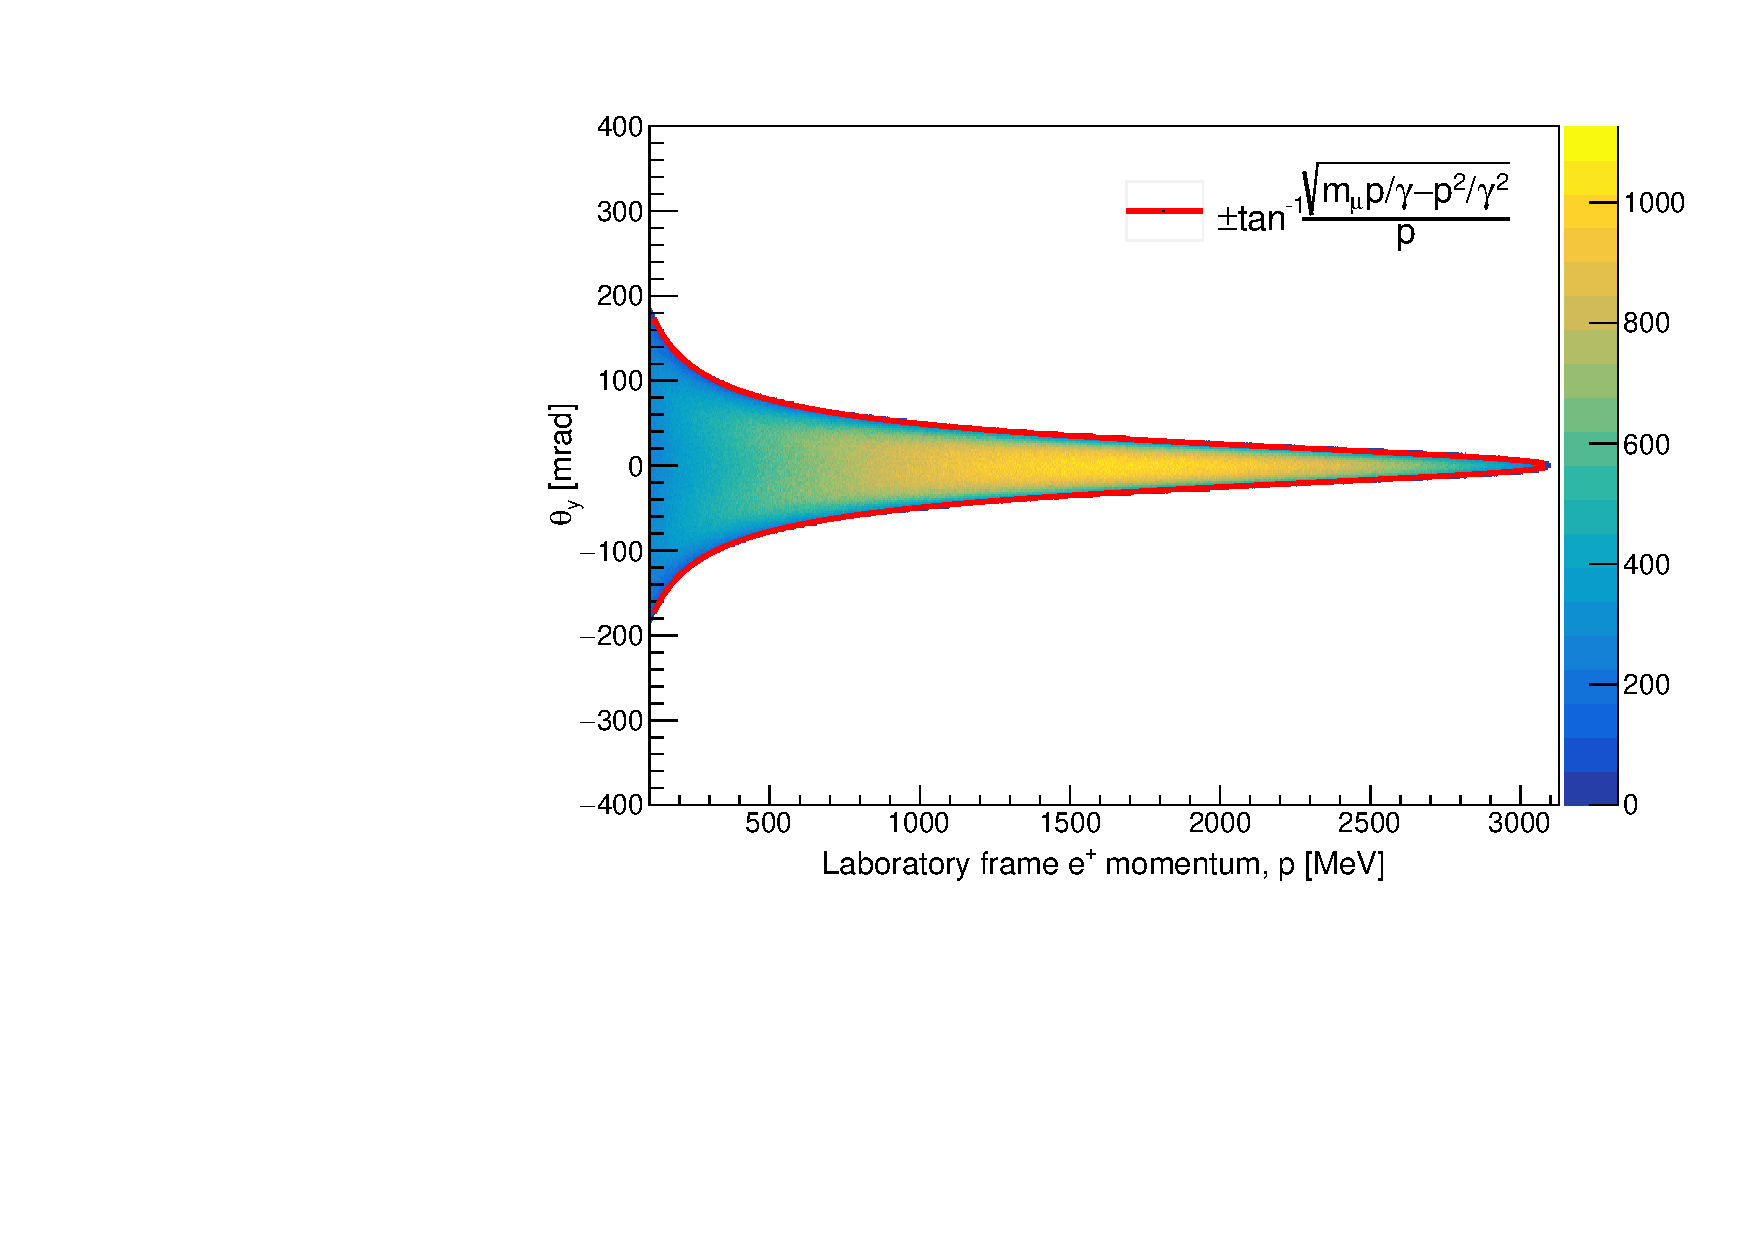
\includegraphics[trim={0 0 0 0},clip,width=.69\textwidth]{Images/Appendix/2DFit.pdf}
\caption{The distribution of laboratory frame vertical angles against momentum, from a simulation sample with complete acceptance and no detector effects. Equation \ref{eqn:MaxVerticalAngle} is overlaid ($\pm \theta_{y}$), showing good agreement with the maximum angles.}
\label{fig:MaxVerticalAngle}
\end{figure}

\chapter[Propagation of errors]{Propagation of errors}\label{app:Unc}

In this appendix, non-trivial expressions for the uncertainties of certain parameters will be derived, utilising the standard formulae for the propagation of errors, which may be found in \cite{Taylor}. For a quantity $z$, comprised of uncorrelated parameters $x$ and $y$, the corresponding uncertainty $\delta z$ is
%
\begin{equation}
  \delta z = \sqrt{\left(\frac{\partial z}{\partial x}\right)^{2}\delta x^{2} + \left(\frac{\partial k}{\partial y}\right)^{2}\delta y^{2}}. %+ 2\frac{\partial k}{\partial m}\frac{\partial k}{\partial c}\sigma_{mc}
  \label{eqn:Taylor9.2}
\end{equation}
%
If $x$ and $y$ are correlated, then $\delta z$ is given by 
\begin{equation}
  \delta z^{2} = \sqrt{\left(\frac{\partial z}{\partial x}\right)^{2}\delta x^{2} + \left(\frac{\partial k}{\partial y}\right)^{2}\delta y^{2} + 2\frac{\partial z}{\partial x}\frac{\partial z}{\partial y}\sigma_{xy}},
  \label{eqn:Taylor9.9}
\end{equation}
%
where $\sigma_{xy}$ is the covariance of $x$ and $y$, defined as
%
\begin{equation}
  \sigma_{xy} = \frac{1}{N}\sum_{i=1}^{N} (x_{i}-\langle x \rangle) (y_{i}-\langle y \rangle).
\end{equation}

\section{The background radial field uncertainty, $\delta \langle B_{r}^{b} \rangle$}\label{app:Brb}

The average background radial field, $\langle B_{r}^{b} \rangle$, is derived from a straight line fit of the form
%
\begin{equation}
  \Delta \langle y \rangle \cdot \Delta V = m\cdot \langle B_{r}^{a} \rangle + c,
\end{equation} 
%
where an example of such a fit is shown in Figure \ref{subfig:PrimaryFieldFit}. $\langle B_{r}^{b} \rangle$ is found at the opposite sign of the $x$-intercept of the fit, where $\Delta \langle y \rangle \cdot \Delta V = 0$, so that
%
\begin{equation}
  \langle B_{r}^{b} \rangle  = \frac{c}{m}.
\end{equation} 
%
Given that the parameters $m$ and $c$ are correlated, Equation \ref{eqn:Taylor9.9} gives the uncertainty 
%
\begin{equation}
% \begin{aligned}
  \delta \langle B_{r}^{b} \rangle^{2} = \left(-\frac{c}{m^{2}}\right)^{2} \delta m^{2}  
   + \left(\frac{1}{m}\right)^{2} \delta c^{2} 
   + 2\left(\frac{1}{m}\right)\left(-\frac{c}{m^{2}}\right)\sigma_{mc}.
% \end{aligned}
\end{equation}
%
Factoring out $\langle B_{r}^{b} \rangle^{2}$ and simplifying, gives 
%
\begin{equation}
  \delta \langle B_{r}^{b} \rangle = \langle B_{r}^{b} \rangle \sqrt{ \left(\frac{\delta m}{m}\right)^{2} + \left(\frac{\delta c}{c}\right)^{2} - \frac{2}{mc}\sigma_{mc} },
\label{eqn:BackgroundBrUnc2}
\end{equation}
%
as given by Equation \ref{eqn:BackgroundBrUnc} in the text.

\section{The radial field conversion factor uncertainty, $\delta k$}\label{app:k}

The constant $k$, required to convert between $\Delta \langle y \rangle$ and $\Delta \langle B_{r} \rangle$, is given by 
%
\begin{equation}
  k = \frac{1}{\frac{m}{V} + c},
  \label{eqn:EmpricalConversionFactor2}
\end{equation}
%
which is reproduced from Equation \ref{eqn:EmpricalConversionFactor}. Given that the fit parameters $m$ and $c$ have some correlation, the uncertainty associated with $k$ follows from Equation \ref{eqn:Taylor9.9}, giving 
%
\begin{equation}
\begin{aligned}
  \delta k^{2} &= \left(-\frac{1}{V}\cdot\frac{1}{(\frac{m}{V}+c)^{2}}\right)^{2}\delta m^{2} \\
  & + \left(-\frac{1}{(\frac{m}{V}+c)^{2}}\right)^{2}\delta c^{2} + \\ 
  & + 2\left(-\frac{1}{V}\cdot\frac{1}{(\frac{m}{V}+c)^{2}}\right)\left(-\frac{1}{(\frac{m}{V}+c)^{2}}\right)\sigma_{mc},
  \label{eqn:DeltaK1}
\end{aligned}
\end{equation}
%
which may to simplified to 
%
\begin{equation}
  \delta k = \sqrt{ \left(\frac{1}{Vk^{2}}\right)^{2}\cdot \delta m^{2} 
  + \left(\frac{1}{k^{4}}\right)\cdot\delta c^{2}
  + \left(\frac{2}{Vk^{4}}\right)\cdot \sigma_{mc} }, 
\end{equation}
%
as given by Equation \ref{eqn:EmpricalConversionFactorError} in the text.

\section{The up/down asymmetry uncertainty, $\delta A$}\label{app:A}

The EDM decay asymmetry, defined in terms of the numbers of simulated `up' and `down' decays, $N_{u}$ and $N_{d}$, as detailed in Chapter \ref{chap:5} Section \ref{sec:DecayAsymVerification}, is defined as 
%
\begin{equation}
  A = \frac{N_{u}-N_{d}}{N_{u}+N_{d}},
  \label{eqn:UpDownAsym2}
\end{equation}
%
by Equation \ref{eqn:UpDownAsym}. Since $N_{u}$ and $N_{d}$ are uncorrelated, Equation \ref{eqn:Taylor9.2} may be applied to determine the corresponding uncertainty, $\delta A$, so that
%
\begin{equation}
  \delta A^{2} = \left(\frac{2N_{d}}{(N_{u}+N_{d})^{2}}\right)^{2}\delta N_{u}^{2} + \left(-\frac{2N_{u}}{(N_{u}+N_{d})^{2}}\right)^{2}\delta N_{d}^{2}. 
  \label{eqn:UpDownAsym3}
\end{equation}
%
Given that the statistical uncertainties, $\delta N_{u}$ and $\delta N_{d}$, are estimated by taking the square root of the central value, so that 
%
\begin{equation}
   \delta N_{u} = \sqrt{N_{u}},
\end{equation}
\begin{equation}
   \delta N_{d} = \sqrt{N_{d}},
\end{equation}
%
then Equation \ref{eqn:UpDownAsym3} may be simplified to
%
\begin{equation}
  \delta A^{2} = \frac{4N_{u}N_{d}}{(N_{u}+N_{d})^{3}} = \frac{1-A^{2}}{N_{u}+N_{d}}, 
\end{equation}
%
which is equivalent to Equation \ref{eqn:UpDownAsymError}. 

\end{appendices}